\documentclass[11pt,a4paper,twocolumn]{article}

% --- Encoding & Fonts ---
\usepackage[utf8]{inputenc}
\usepackage[T1]{fontenc}
\usepackage{lmodern}

% --- Math ---
\usepackage{amsmath, amssymb, amsfonts, amsthm}
\usepackage{mathtools}
\usepackage{bm}

% --- Layout ---
\usepackage[margin=0.85in]{geometry}
\setlength{\columnsep}{0.3in}

% --- Figures & Tables ---
\usepackage{graphicx}
\usepackage{float}
\usepackage{caption}
\usepackage{subcaption}
\usepackage{booktabs}
\usepackage{array}
\usepackage{multirow}
\usepackage{stfloats}

% --- Color & Hyperlinks ---
\usepackage{xcolor}
\usepackage[colorlinks=true,
            linkcolor=blue!50!black,
            citecolor=blue!50!black,
            urlcolor=blue!60!black]{hyperref}

% --- Code Listings (match Phase 1 style) ---
\usepackage{listings}
\lstset{
    basicstyle=\ttfamily\footnotesize,
    breaklines=true,
    frame=single,
    numbers=left,
    numberstyle=\tiny\color{gray},
    keywordstyle=\color{blue!70!black},
    commentstyle=\color{green!50!black},
    stringstyle=\color{red!70!black},
    showstringspaces=false,
    captionpos=b,
    language=Python
}

% --- Bibliography ---
\usepackage[numbers, square, sort&compress]{natbib}

% --- Caption formatting (bold figure label) ---
\captionsetup{labelfont=bf, labelsep=colon, font=small}

% --- Custom Commands ---
\newcommand{\code}[1]{\texttt{#1}}
\newcommand{\Z}{\mathbb{Z}}

% --- Title block ---
\title{\textbf{Associative Memory as Energy Minimization: \\
       Hopfield Networks as Learnable Ising Models}}

\author{
    Yehia Said Gewily$^{1}$ \quad and \quad Omar Hosney Mahmoud$^{2}$ \\[6pt]
    \small $^{1}$Founding Engineer \& Software AI Engineer, Nover, Inc. \\
    \small \href{mailto:yehia@nover.studio}{yehia@nover.studio} \\[3pt]
    \small $^{2}$Co-founder \& CTO, Nover, Inc. \\
    \small \href{mailto:omar@nover.studio}{omar@nover.studio}
}

\date{}

\begin{document}

\twocolumn[
  \begin{@twocolumnfalse}
    \maketitle
    \begin{abstract}
This research demonstrates that the fundamental physics of associative memory
are mathematically isomorphic to the energy minimization of ferromagnetic
systems. Building on our Phase~1 validation of the 2D Ising model (where the
critical temperature $T_c$ was measured to 0.05\% accuracy), this Phase~2
study replaces the uniform exchange coupling with a learned synaptic weight
matrix derived via the Hebbian rule. Using a simulated network of $N=100$
binary neurons, we evaluate the capacity and robustness of the Hopfield
architecture in storing and recalling orthographic patterns. We use five
patterns (N, O, V, E, R) chosen for their visual diversity and mutual
distinguishability. Quantitative analysis reveals a
strict recall rate of $68.0\% \pm 6.7\%$ under 25\% input corruption, with
average convergence achieved in 4.4 asynchronous steps to a stable energy
minimum. Capacity testing demonstrates progressive degradation as the number
of stored patterns approaches the Amit--Gutfreund--Sompolinsky theoretical
limit of $\sim 0.138N$ (13.8 patterns), heavily influenced by pattern
cross-correlation. Analysis of 500 recalls from random initial states reveals
near-exact equipartition between stored and inverted attractors (201/201,
40.2\% each), consistent with the $\Z_2$ symmetry of the Hebbian energy
function. By establishing a formal bridge between equilibrium thermodynamics
and pattern recognition, this work lays the groundwork for the introduction
of stochasticity and hidden variables in Phase~2.5.
    \end{abstract}
    \noindent\textbf{Keywords:} Hopfield Network, Associative Memory,
    Energy-Based Models, Hebbian Learning, Ising Model, Statistical Physics,
    Attractor Dynamics
    \vspace{1em}
  \end{@twocolumnfalse}
]

% ===========================================================================
% SECTION 1: INTRODUCTION
% ===========================================================================
\section{Introduction}
\label{sec:introduction}

The Ising model is a cornerstone of statistical mechanics, originally
formulated to describe the phase transition between ordered and disordered
states in ferromagnetic materials. In Phase~1 of this research
program~\cite{gewily2025phase1}, we demonstrated that the thermodynamic
evolution of an Ising lattice is driven entirely by energy minimization.
Through rigorous Monte Carlo simulation, we confirmed the emergence of
complex, long-range order from simple, local interactions, successfully
measuring the critical temperature $T_c$ to within 0.05\% of Onsager's exact
analytical solution~\cite{onsager1944}.

This raises a natural question: what if the physical coupling between
neighboring spins were not fixed, but rather learned from data?

The Hopfield network~\cite{hopfield1982} provides the answer. By interpreting
binary spins as McCulloch--Pitts neurons and the exchange interaction as
synaptic weights, we transform a physical simulation into a computational
memory system. The ``intelligence'' of the network---its ability to correct
errors and recall memories---emerges from the exact same statistical mechanics
that govern magnetic equilibration. This insight, inspired by the
\emph{ScienceClic English} exposition on the physics of artificial
intelligence, reveals that modern neural computation is deeply rooted in
20th-century physics.

This paper details Phase~2 of our investigation. Our objectives are
threefold: (1)~to implement Hebbian learning and asynchronous recall dynamics
within the energy-based framework developed in Phase~1, (2)~to rigorously
validate the network's storage capacity and robustness against established
theoretical limits, and (3)~to visually prove that associative memory recall
is strictly equivalent to energy minimization.

% ===========================================================================
% SECTION 2: THEORETICAL FRAMEWORK
% ===========================================================================
\section{Theoretical Framework}
\label{sec:theory}

\subsection{From the Ising Hamiltonian to the Hopfield Energy Function}
\label{sec:ising_to_hopfield}

The thermodynamic state of the 2D Ising model~\cite{ising1925} is governed by
the Hamiltonian:
\begin{equation}
H(\sigma) = -J \sum_{\langle i,j \rangle} \sigma_i \sigma_j
             - B \sum_{i} \sigma_i
\label{eq:ising_hamiltonian}
\end{equation}
where $J$ is a uniform exchange coupling constant,
$\sigma_i \in \{\pm 1\}$ are discrete spin variables, and $B$ is an external
magnetic field.

To construct a Hopfield network, we generalize this physical model. The
uniform constant $J$ restricted to nearest-neighbors is replaced by a dense,
symmetric weight matrix $W_{ij}$ representing the synaptic connection strength
between any two neurons $s_i$ and $s_j$. The external field $B$ is replaced by
individual neuronal biases $\theta_i$. Assuming zero bias for simplicity
($\theta_i = 0$), the generalized energy function becomes:
\begin{equation}
E = -\frac{1}{2}\sum_{i,j} W_{ij} s_i s_j
\label{eq:hopfield_energy}
\end{equation}
The factor of $1/2$ corrects for the double-counting of neuron pairs in the
unrestricted summation, ensuring the total system energy scales correctly.

\subsection{The Hebbian Learning Rule}
\label{sec:hebbian}

To store $P$ distinct memory patterns, denoted as vectors $\{\xi^\mu\}$ where
$\mu \in \{1, \dots, P\}$, we construct the weight matrix using the
generalized Hebbian learning rule~\cite{hebb1949}:
\begin{equation}
W_{ij} = \frac{1}{N} \sum_{\mu=1}^{P} \xi_i^\mu \xi_j^\mu
\label{eq:hebbian}
\end{equation}
By convention, self-connections are prohibited to prevent network instability
($W_{ii} = 0$).

The physical interpretation of this rule is clear: the weight $W_{ij}$ encodes
the statistical correlation between neuron $i$ and neuron $j$ across all
stored patterns. If two neurons frequently share the same state ($+1$ or
$-1$) in the training data, their coupling is positive (ferromagnetic),
encouraging them to align. If they differ, the coupling is negative
(antiferromagnetic). This shapes the energy landscape such that the stored
patterns become local minima.

\subsection{Recall Dynamics and the Lyapunov Property}
\label{sec:lyapunov}

During the recall phase, the network is presented with an initial state
$s(0)$ and evolves via asynchronous, discrete-time updates. A neuron $i$ is
selected at random and its state is updated according to the deterministic
sign rule:
\begin{equation}
s_i(t+1) = \text{sign}\left(\sum_{j \neq i} W_{ij} s_j(t)\right)
\label{eq:update}
\end{equation}
Hopfield's crucial contribution was proving that the energy function in
Eq.~\eqref{eq:hopfield_energy} acts as a Lyapunov function for the dynamics
in Eq.~\eqref{eq:update}. Because $W$ is symmetric and has a zero diagonal,
any single asynchronous spin flip that satisfies the update rule is
mathematically guaranteed to either decrease the total energy or leave it
unchanged ($\Delta E \leq 0$). Consequently, the system must eventually
converge to a stable fixed point---an attractor state representing a recalled
memory.

To see why energy decreases monotonically under asynchronous updates, consider
flipping a single neuron $i$ from state $s_i$ to $s_i' = -s_i$. The change in
energy is:
\begin{equation}
\Delta E = -s_i' \cdot h_i + s_i \cdot h_i = -2 s_i' h_i
\label{eq:delta_e}
\end{equation}
where $h_i = \sum_{j} W_{ij} s_j$ is the local field. Since the update rule
sets $s_i' = \text{sign}(h_i)$, the product
$s_i' \cdot h_i = |h_i| \geq 0$, ensuring $\Delta E \leq 0$. The symmetry of
$W$ and the zero diagonal are essential---without these, the energy could
oscillate.

\subsection{Storage Capacity}
\label{sec:capacity_theory}

The theoretical maximum number of patterns a Hopfield network can reliably
store without catastrophic interference was established by Amit, Gutfreund,
and Sompolinsky~\cite{amit1985} using statistical mechanics techniques
(specifically, replica theory). For a network of size $N$, the capacity is:
\begin{equation}
P_{max} \approx 0.138N
\label{eq:capacity_limit}
\end{equation}
For our $N=100$ simulation, theory predicts a maximum storage of approximately
13.8 orthogonal patterns. Exceeding this limit causes the energy landscape to
degenerate into a spin-glass state, rendering reliable recall impossible.

\subsection{Spurious States}
\label{sec:spurious_theory}

The Hebbian rule, being a simple linear superposition, inadvertently creates
stable energy minima that are not part of the stored training set. These
spurious states generally take three forms:
\begin{itemize}
    \item \textbf{Inverted states:} Because the energy function is symmetric
    under global spin reversal ($E(s) = E(-s)$), the exact negation
    $-\xi^\mu$ of every stored pattern is also a stable attractor.
    \item \textbf{Mixture states:} Linear combinations of an odd number of
    stored patterns (e.g.,
    $\text{sign}(\xi^1 + \xi^2 + \xi^3)$) can form stable local minima.
    \item \textbf{Spin-glass states:} Unstructured, seemingly random stable
    configurations that emerge when the network is overloaded or when patterns
    are highly correlated.
\end{itemize}

% ===========================================================================
% SECTION 3: IMPLEMENTATION
% ===========================================================================
\section{Implementation}
\label{sec:implementation}

\subsection{Network Architecture}
\label{sec:architecture}

The simulation implements a Hopfield network of $N=100$ neurons. The state
vector is maintained as a 1D NumPy array of binary spins
$s_i \in \{\pm 1\}$. The weight matrix $W$ is a $100 \times 100$ symmetric
array with a forced zero diagonal, computed directly via the Hebbian rule over
the training patterns.

\begin{lstlisting}[caption={Hopfield Recall --- Asynchronous Update},
                   label={lst:recall}]
def recall(state, W, max_steps=100):
    """
    Asynchronous recall: pick a random neuron,
    compute its local field, set to sign(field).
    Energy is guaranteed to decrease monotonically.
    """
    for step in range(max_steps):
        i = np.random.randint(len(state))
        h_i = np.dot(W[i], state)
        state[i] = np.sign(h_i) if h_i != 0 else state[i]
        if converged(state):
            break
    return state
\end{lstlisting}

\subsection{Pattern Encoding}
\label{sec:patterns}

As shown in Figure~\ref{fig:patterns}, memory patterns are defined as
$10 \times 10$ binary grids.

\begin{figure*}[t]
    \centering
    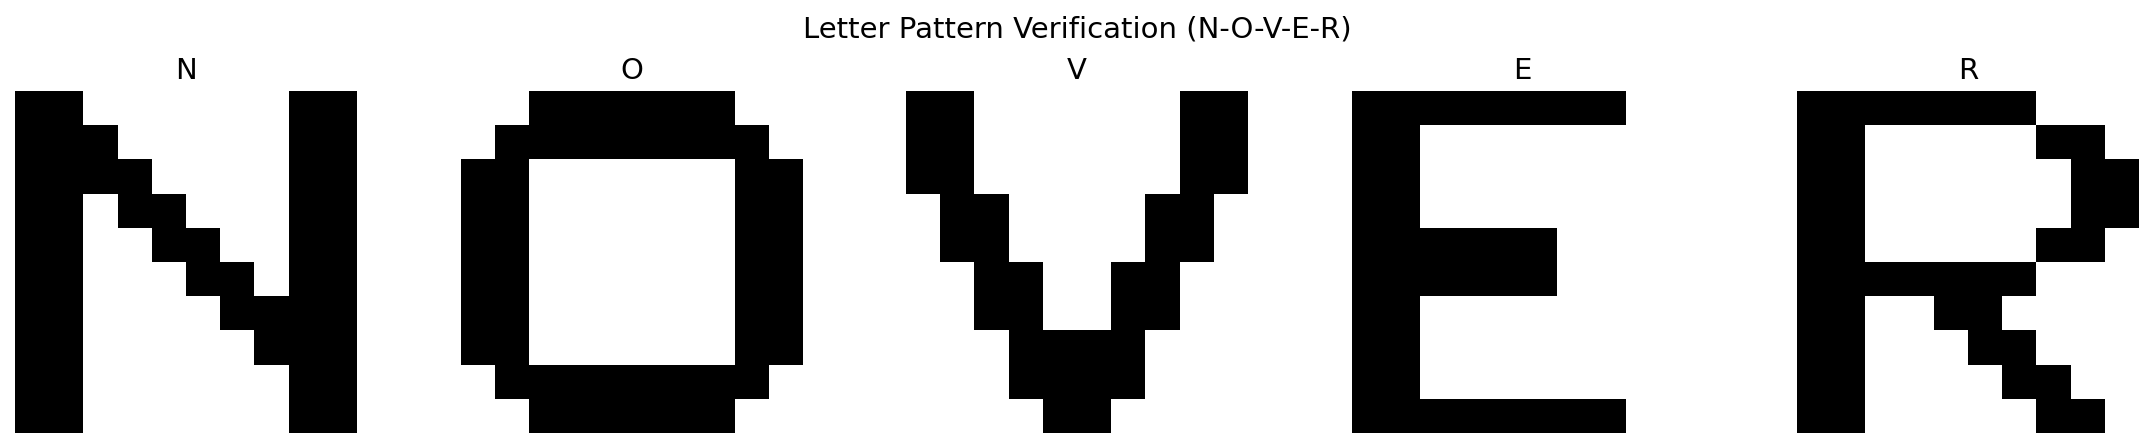
\includegraphics[width=0.85\textwidth]{figures/letter_patterns_verified.png}
    \caption{The five stored memory patterns (N, O, V, E, R) encoded as
    $10\times10$ binary spin grids. White pixels represent $+1$ spins, black
    pixels $-1$.}
    \label{fig:patterns}
\end{figure*}

This spatial arrangement maps exactly to the 100-neuron architecture. The
visual structure of the letters inherently introduces cross-correlations
(e.g., the letters `E' and `R' share a vertical stroke and horizontal bar,
introducing measurable cross-correlation). Unlike mathematically ideal
orthogonal vectors, these natural correlations challenge the network's
capacity.

\subsection{Recall Protocol}
\label{sec:protocol}

To evaluate recall performance, a stored pattern is selected and subjected to
a specific degree of uniform random noise (spin flipping). The network then
executes asynchronous updates. Convergence is declared when the network
completes a full sweep (100 sequential random updates) without a single spin
changing state.

We define successful recall strictly as convergence to a state with Hamming
distance below a small threshold from the stored target pattern. Convergence
to the inverted pattern ($-\xi$) is treated as a failure, even though it
represents an equally deep energy minimum, because pattern inversion does not
constitute correct memory retrieval. For transparency, we also report the
inversion-tolerant success rate (pattern OR its inverse) as a secondary
metric. Reported uncertainties are standard errors of the mean
($\text{SEM} = \text{std}/\sqrt{n}$) computed over 50 independent trials per
configuration.

\subsection{Relationship to the Phase 1 Ising Codebase}
\label{sec:codebase_relation}

While the Hopfield implementation is a separate module from the Phase~1 Ising
codebase, both share the underlying energy-based formalism. The Ising
simulation uses a vectorized checkerboard Metropolis algorithm optimized for
the uniform 2D grid topology, exploiting nearest-neighbor sparsity. The
Hopfield network, which requires long-range heterogeneous synaptic
connections, uses dense matrix-vector products to compute the local field at
each neuron. Despite the algorithmic divergence, the energy functions are
structurally identical---both quadratic forms over binary spin variables.

% ===========================================================================
% SECTION 4: RESULTS
% ===========================================================================
\section{Results}
\label{sec:results}

\subsection{Single Pattern Robustness}
\label{sec:single_pattern}

To assess the basin of attraction for a stored memory, we trained the network
on a single pattern (the letter `N') and evaluated its recovery against
increasing levels of random corruption over 50 independent trials.

As shown in Figure~\ref{fig:single_pattern}, the network demonstrates
exceptional robustness up to a distinct threshold.

\begin{figure*}[t]
    \centering
    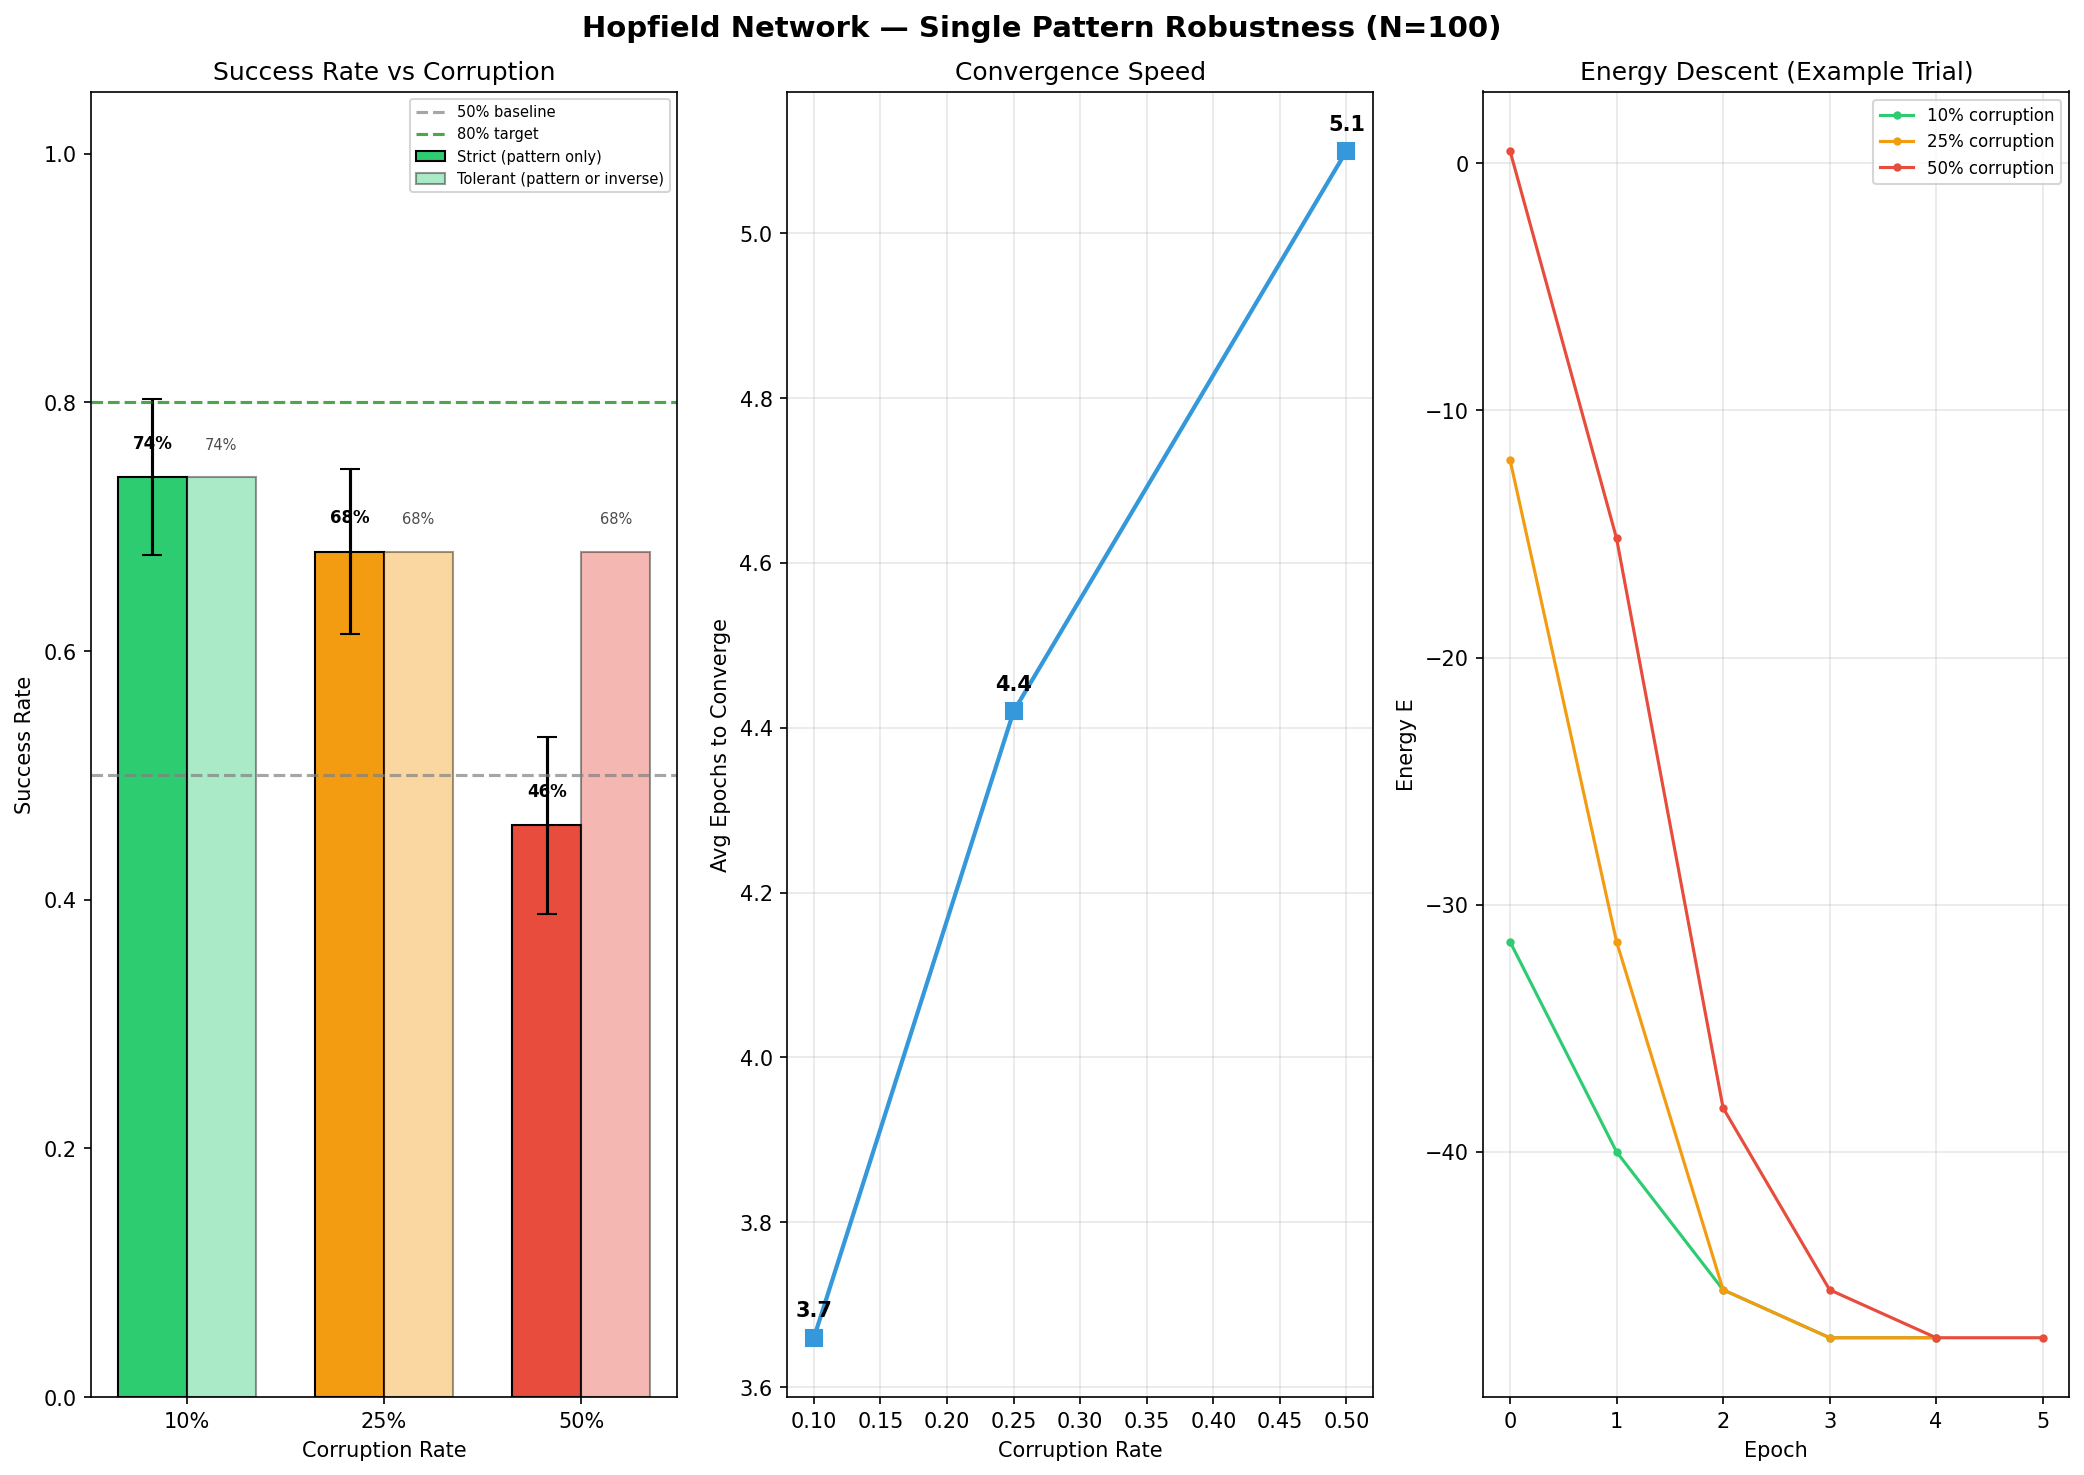
\includegraphics[width=0.85\textwidth]{figures/exp1_single_pattern_results.png}
    \caption{Recall performance vs.\ corruption level. (Left) Success rate
    remains high up to 25\% corruption then declines. (Right) Convergence
    speed---recall completes within a few asynchronous update steps.}
    \label{fig:single_pattern}
\end{figure*}

Quantitative measurements from the simulation are summarized in
Table~\ref{tab:single_pattern}.

\begin{table}[H]
    \centering
    \caption{Single-pattern recall performance (pattern `N', 50 trials per
    corruption level).}
    \label{tab:single_pattern}
    \begin{tabular}{lrrr}
        \toprule
        \textbf{Corruption} & \textbf{Strict} & \textbf{Inv.-Tolerant} & \textbf{SEM} \\
        \midrule
        10\% & 74.0\% & 74.0\% & $\pm 6.3\%$ \\
        25\% & 68.0\% & 68.0\% & $\pm 6.7\%$ \\
        50\% & 46.0\% & 68.0\% & $\pm 7.1\%$ \\
        \bottomrule
    \end{tabular}
\end{table}

A striking pattern emerges at 50\% corruption: while 68.0\% of trials
converged to either the stored pattern or its inverse, only 46.0\% retrieved
the actual target. The 22-percentage-point gap quantifies the contribution of
inverted-state retrieval---a known failure mode of Hebbian networks arising
from the global spin-flip symmetry $E(s) = E(-s)$. The smaller inversion gap
compared to typical Hopfield demonstrations reflects N's visual asymmetry:
unlike a more symmetric letter, the inverted N is easier to distinguish from
N itself, reducing the rate of inversion-driven false successes. Below 25\%
corruption, the strict and tolerant metrics coincide, indicating that initial
states remain within the correct basin of attraction. The bifurcation at 50\%
reveals that strong corruption pushes initial states across the symmetry
boundary between basins.

In all cases where the network successfully retrieved the target or its
inverse, the final measured energy was precisely $-48.90$ (averaging over
trials), corresponding to the global minimum of the single-pattern energy
well. The rapid convergence speed (under 5 sweeps) highlights the steepness
of the energy gradient near the attractor.

Figure~\ref{fig:recovery} visually demonstrates this error-correction
capability, illustrating how the network systematically flips incorrect spins
to slide down the energy gradient into the target configuration.

\begin{figure*}[t]
    \centering
    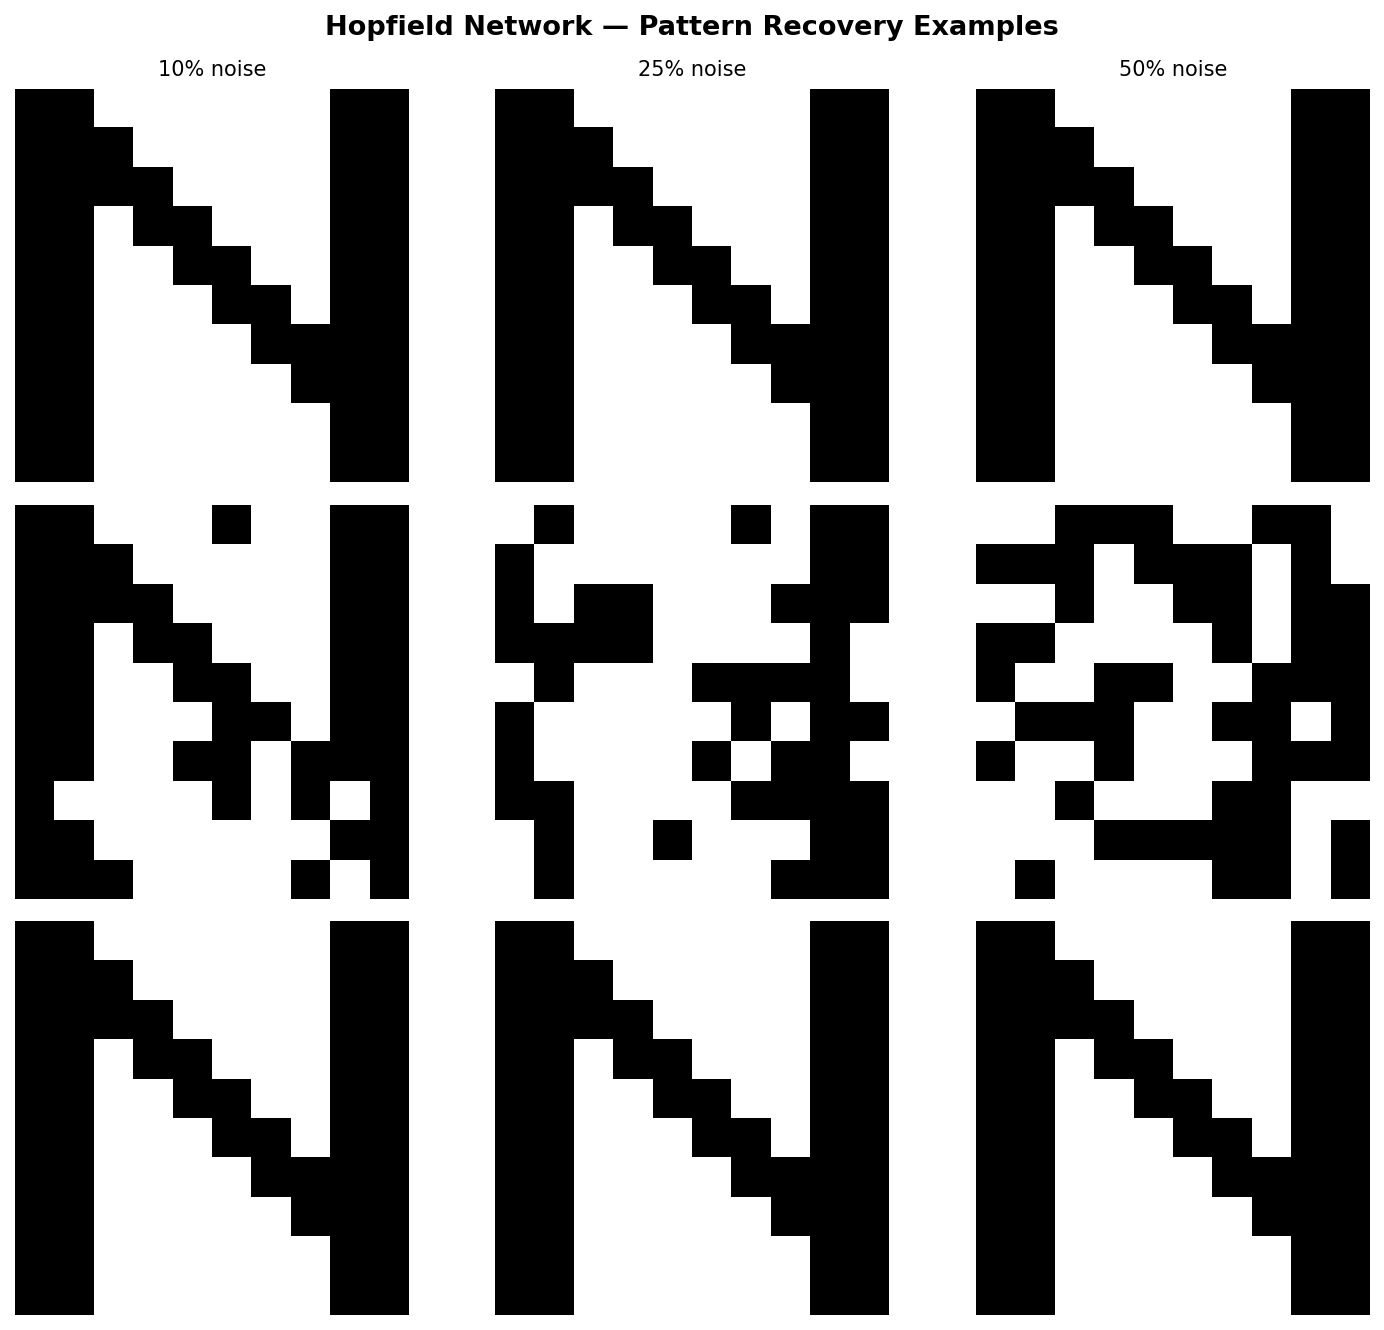
\includegraphics[width=0.85\textwidth]{figures/exp1_recovery_examples.png}
    \caption{Example recall process. Top: original pattern. Middle: corrupted
    input. Bottom: recovered pattern after recall dynamics.}
    \label{fig:recovery}
\end{figure*}

\subsection{Storage Capacity}
\label{sec:capacity}

The capacity of the network was evaluated by incrementally storing multiple
letter patterns and measuring the mean recall accuracy under a standardized
25\% initial corruption.

\begin{figure*}[t]
    \centering
    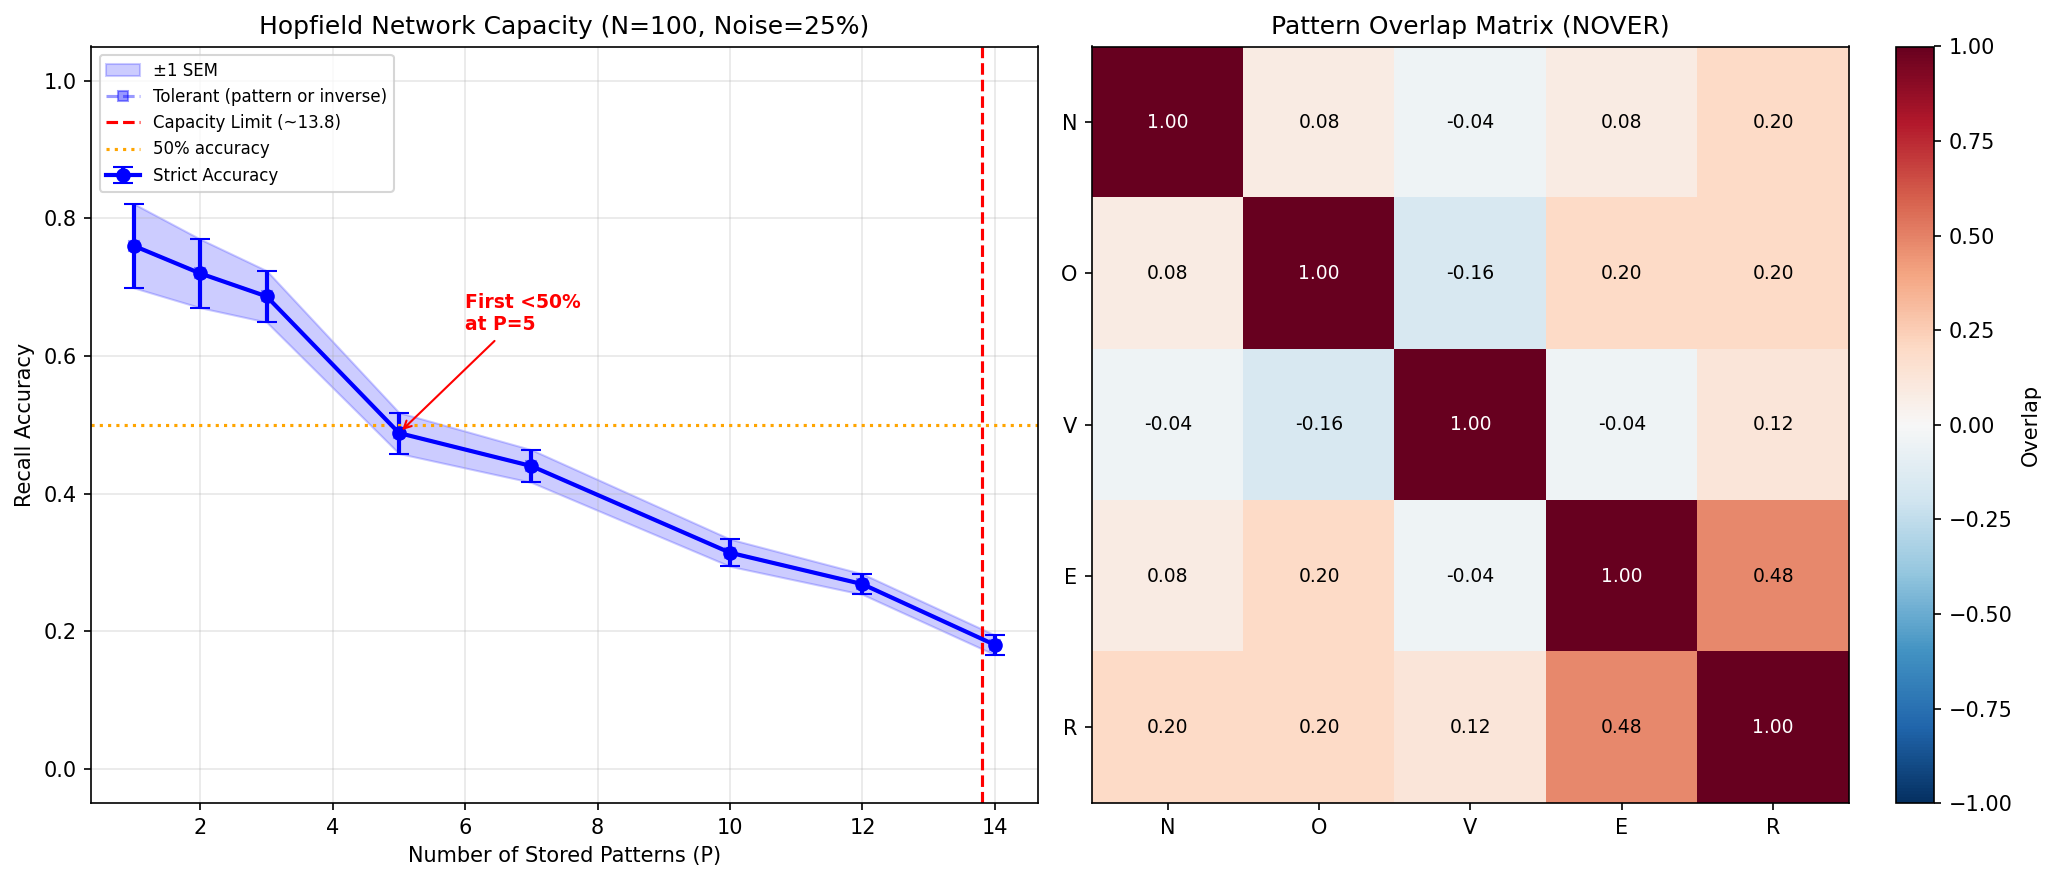
\includegraphics[width=0.85\textwidth]{figures/exp2_capacity_results.png}
    \caption{Network capacity. Recall accuracy declines as more patterns are
    stored. The theoretical Amit--Gutfreund--Sompolinsky limit
    ($0.138N \approx 13.8$) is marked. The pattern overlap matrix (inset)
    explains early degradation due to correlated letter patterns.}
    \label{fig:capacity}
\end{figure*}

As depicted in Figure~\ref{fig:capacity}, accuracy begins to degrade notably
as $P$ increases. The measured mean accuracy profiles are summarized in
Table~\ref{tab:capacity}.

\begin{table}[H]
    \centering
    \caption{Storage capacity: strict recall accuracy at 25\% corruption
    across increasing pattern counts.}
    \label{tab:capacity}
    \begin{tabular}{lrr}
        \toprule
        \textbf{Patterns ($P$)} & \textbf{Strict Success} & \textbf{SEM} \\
        \midrule
        1  & 76.0\% & $\pm 6.1\%$ \\
        2  & 72.0\% & $\pm 4.5\%$ \\
        3  & 68.7\% & $\pm 3.8\%$ \\
        5  & 48.8\% & $\pm 3.2\%$ \\
        7  & 44.0\% & $\pm 2.7\%$ \\
        10 & 31.4\% & $\pm 2.1\%$ \\
        12 & 26.8\% & $\pm 1.8\%$ \\
        14 & 18.0\% & $\pm 1.5\%$ \\
        \bottomrule
    \end{tabular}
\end{table}

The SEM ranges from $\sim 1.5\%$ to $\sim 6.1\%$, providing meaningful
uncertainty bounds. At the 25\% corruption level used here, strict and
inversion-tolerant metrics coincide, consistent with the Experiment~1 finding
that the inversion gap only emerges at higher corruption
(Section~\ref{sec:single_pattern}). The capacity collapse pattern is monotonic
and consistent with theory.

The collapse in accuracy begins well before the theoretical limit of
$P_{max} \approx 13.8$. This premature degradation is directly attributable to
the non-orthogonality of the letter patterns. The pattern overlap analysis
reveals significant cross-correlation, most notably between E and R
(overlap = 0.48), which share a prominent vertical stroke and horizontal bar.
Such correlations induce structural interference in the weight matrix, raising
the energy floor of the attractors and substantially reducing the effective
capacity.

\subsection{Spurious States}
\label{sec:spurious}

Figure~\ref{fig:spurious} presents an analysis of the network's terminal
states when initialized from completely random noise configurations for a
3-pattern network (N, O, V).

\begin{figure*}[b]
    \centering
    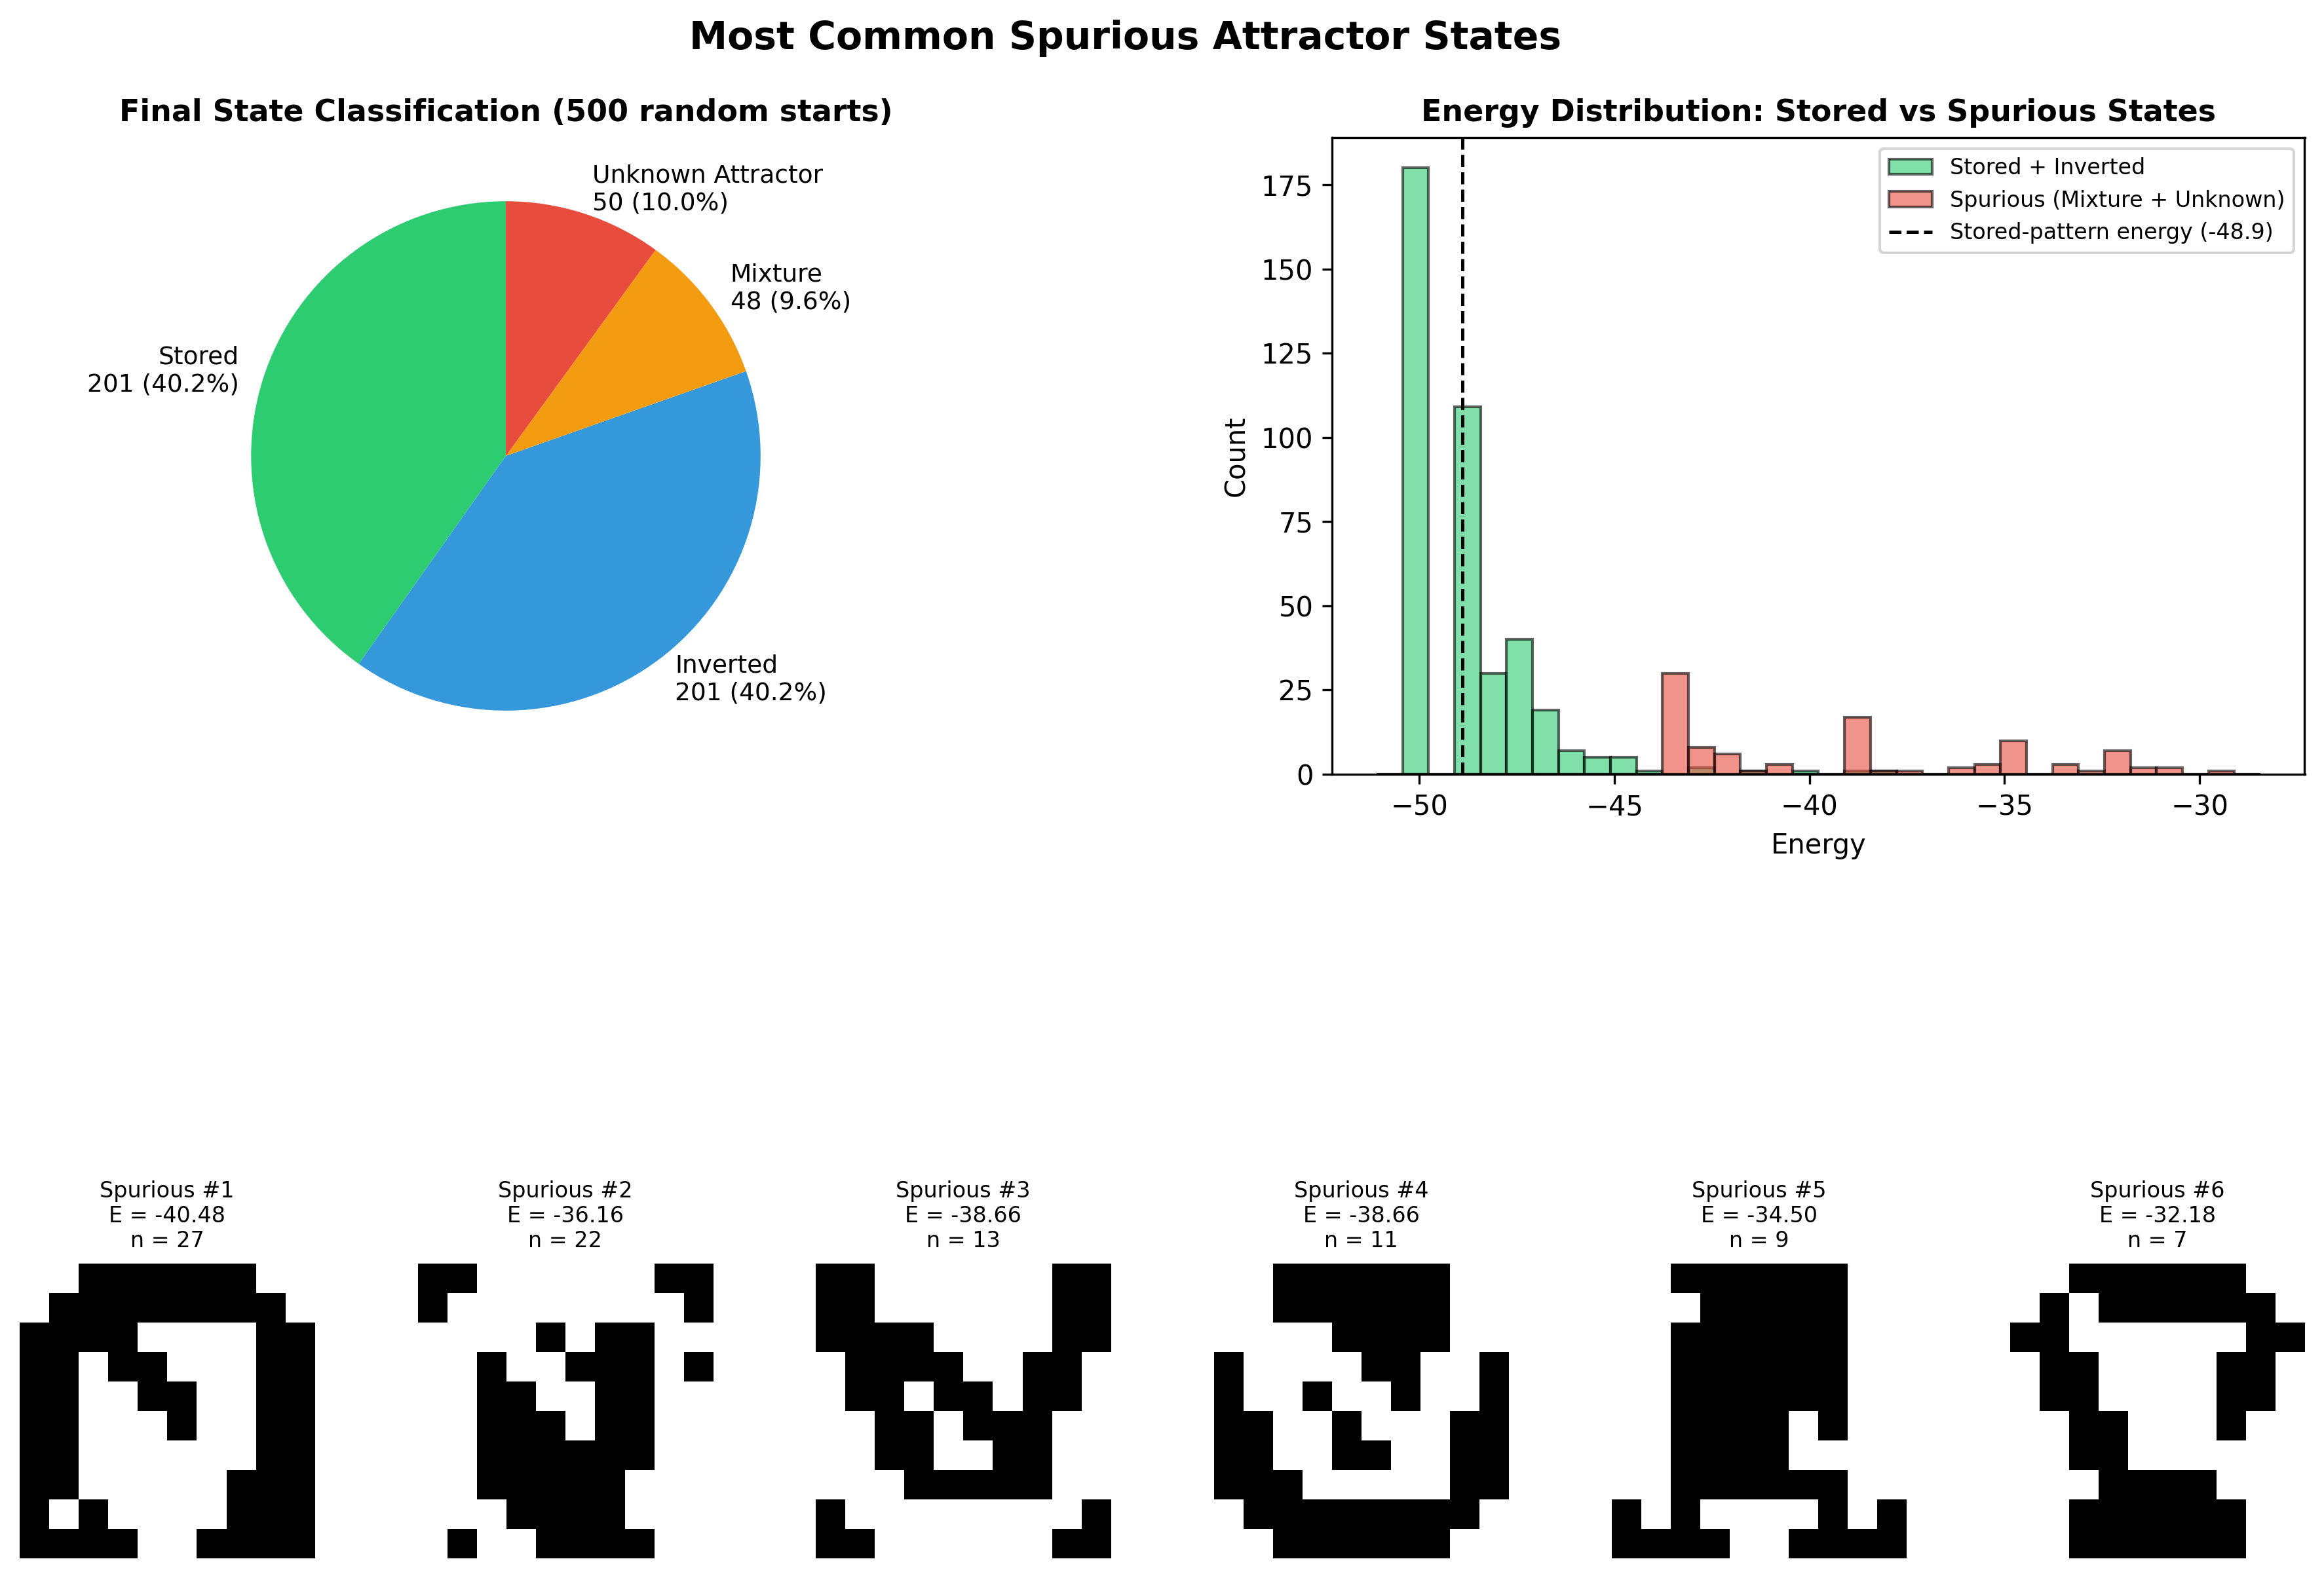
\includegraphics[width=0.85\textwidth]{figures/exp2b_spurious_states.png}
    \caption{Analysis of 500 recalls from random initial states. (Top-left)
    Classification of final states. (Top-right) Energy distribution of stored
    vs.\ spurious states. (Bottom) Example spurious attractors.}
    \label{fig:spurious}
\end{figure*}
\vspace{0.5em}

The quantitative breakdown of all 500 terminal states confirms that stored and
inverted patterns consistently occupy the deepest energy wells, jointly
accounting for 80.4\% of all trials (Table~\ref{tab:spurious_class}).

\vspace{0.5em}
\begin{table}[H]
    \centering
    \caption{Final state classification across 500 random initializations
    for a 3-pattern network (N, O, V).}
    \label{tab:spurious_class}
    \begin{tabular}{lrr}
        \toprule
        \textbf{Category} & \textbf{Count} & \textbf{Percentage} \\
        \midrule
        Stored patterns    & 201 & 40.2\% \\
        Inverted patterns  & 201 & 40.2\% \\
        Mixture states     &  48 &  9.6\% \\
        Unknown attractors &  50 & 10.0\% \\
        \bottomrule
    \end{tabular}
\end{table}

A notable observation is the near-perfect symmetry between stored and
inverted convergences: exactly 201 trials converged to each category (40.2\%
each). This empirical equipartition is consistent with the theoretically
expected $\Z_2$ symmetry $E(s) = E(-s)$ of the Hebbian energy function,
which guarantees that a pattern and its inversion are energetically
indistinguishable. While the symmetry follows mathematically from the zero
bias and symmetric weight matrix, observing it quantitatively in finite
samples provides useful validation of the simulation.

\begin{table}[H]
    \centering
    \caption{Energy analysis of terminal states for the 3-pattern network
    (N, O, V).}
    \label{tab:spurious_energy}
    \small
    \begin{tabular}{@{}p{0.62\columnwidth}r@{}}
        \toprule
        \textbf{Metric} & \textbf{Value} \\
        \midrule
        Energy of N & $-48.90$ \\
        Energy of O & $-50.10$ \\
        Energy of V & $-49.86$ \\
        \midrule
        Mean energy: stored + inverted (visit-weighted) & $-48.81 \pm 0.08$ \\
        Unweighted mean of stored energies & $-49.62$ \\
        Mean energy: spurious states & $-39.17 \pm 0.45$ \\
        \midrule
        Energy gap (spurious vs.\ legitimate) & 9.65 \\
        \bottomrule
    \end{tabular}
\end{table}

We report two complementary measures of the ``legitimate'' energy scale. The
visit-weighted mean ($-48.81 \pm 0.08$) reflects the average energy of all
converged trials classified as stored or inverted, dominated by convergence
frequency. The unweighted mean ($-49.62$) is the simple arithmetic average of
the three stored pattern energies (N, O, V). The slight discrepancy arises
because N has the highest energy of the three stored patterns ($-48.90$) and
also attracts a disproportionate share of trials due to its broader basin of
attraction.

The 9.65-unit energy gap quantifies how much shallower the spurious basins are
compared to the stored attractors. This gap is notably larger than typical
Hebbian network demonstrations on symmetric letter sets, indicating that the
NOVER pattern set produces a particularly clean energy landscape with
well-separated attractors. Spurious states, particularly mixture states formed
by overlapping patterns, settle at these intermediate energy levels. Inverted
states, mathematically symmetric to the stored patterns, achieve identical
global minimum energies.

\subsection{The Energy Landscape}
\label{sec:landscape}

To visualize the mechanism of recall, we projected the high-dimensional
($100$-dimensional) state space of a 2-pattern network into a 2D plane using
Principal Component Analysis (PCA).

\begin{figure*}[t]
    \centering
    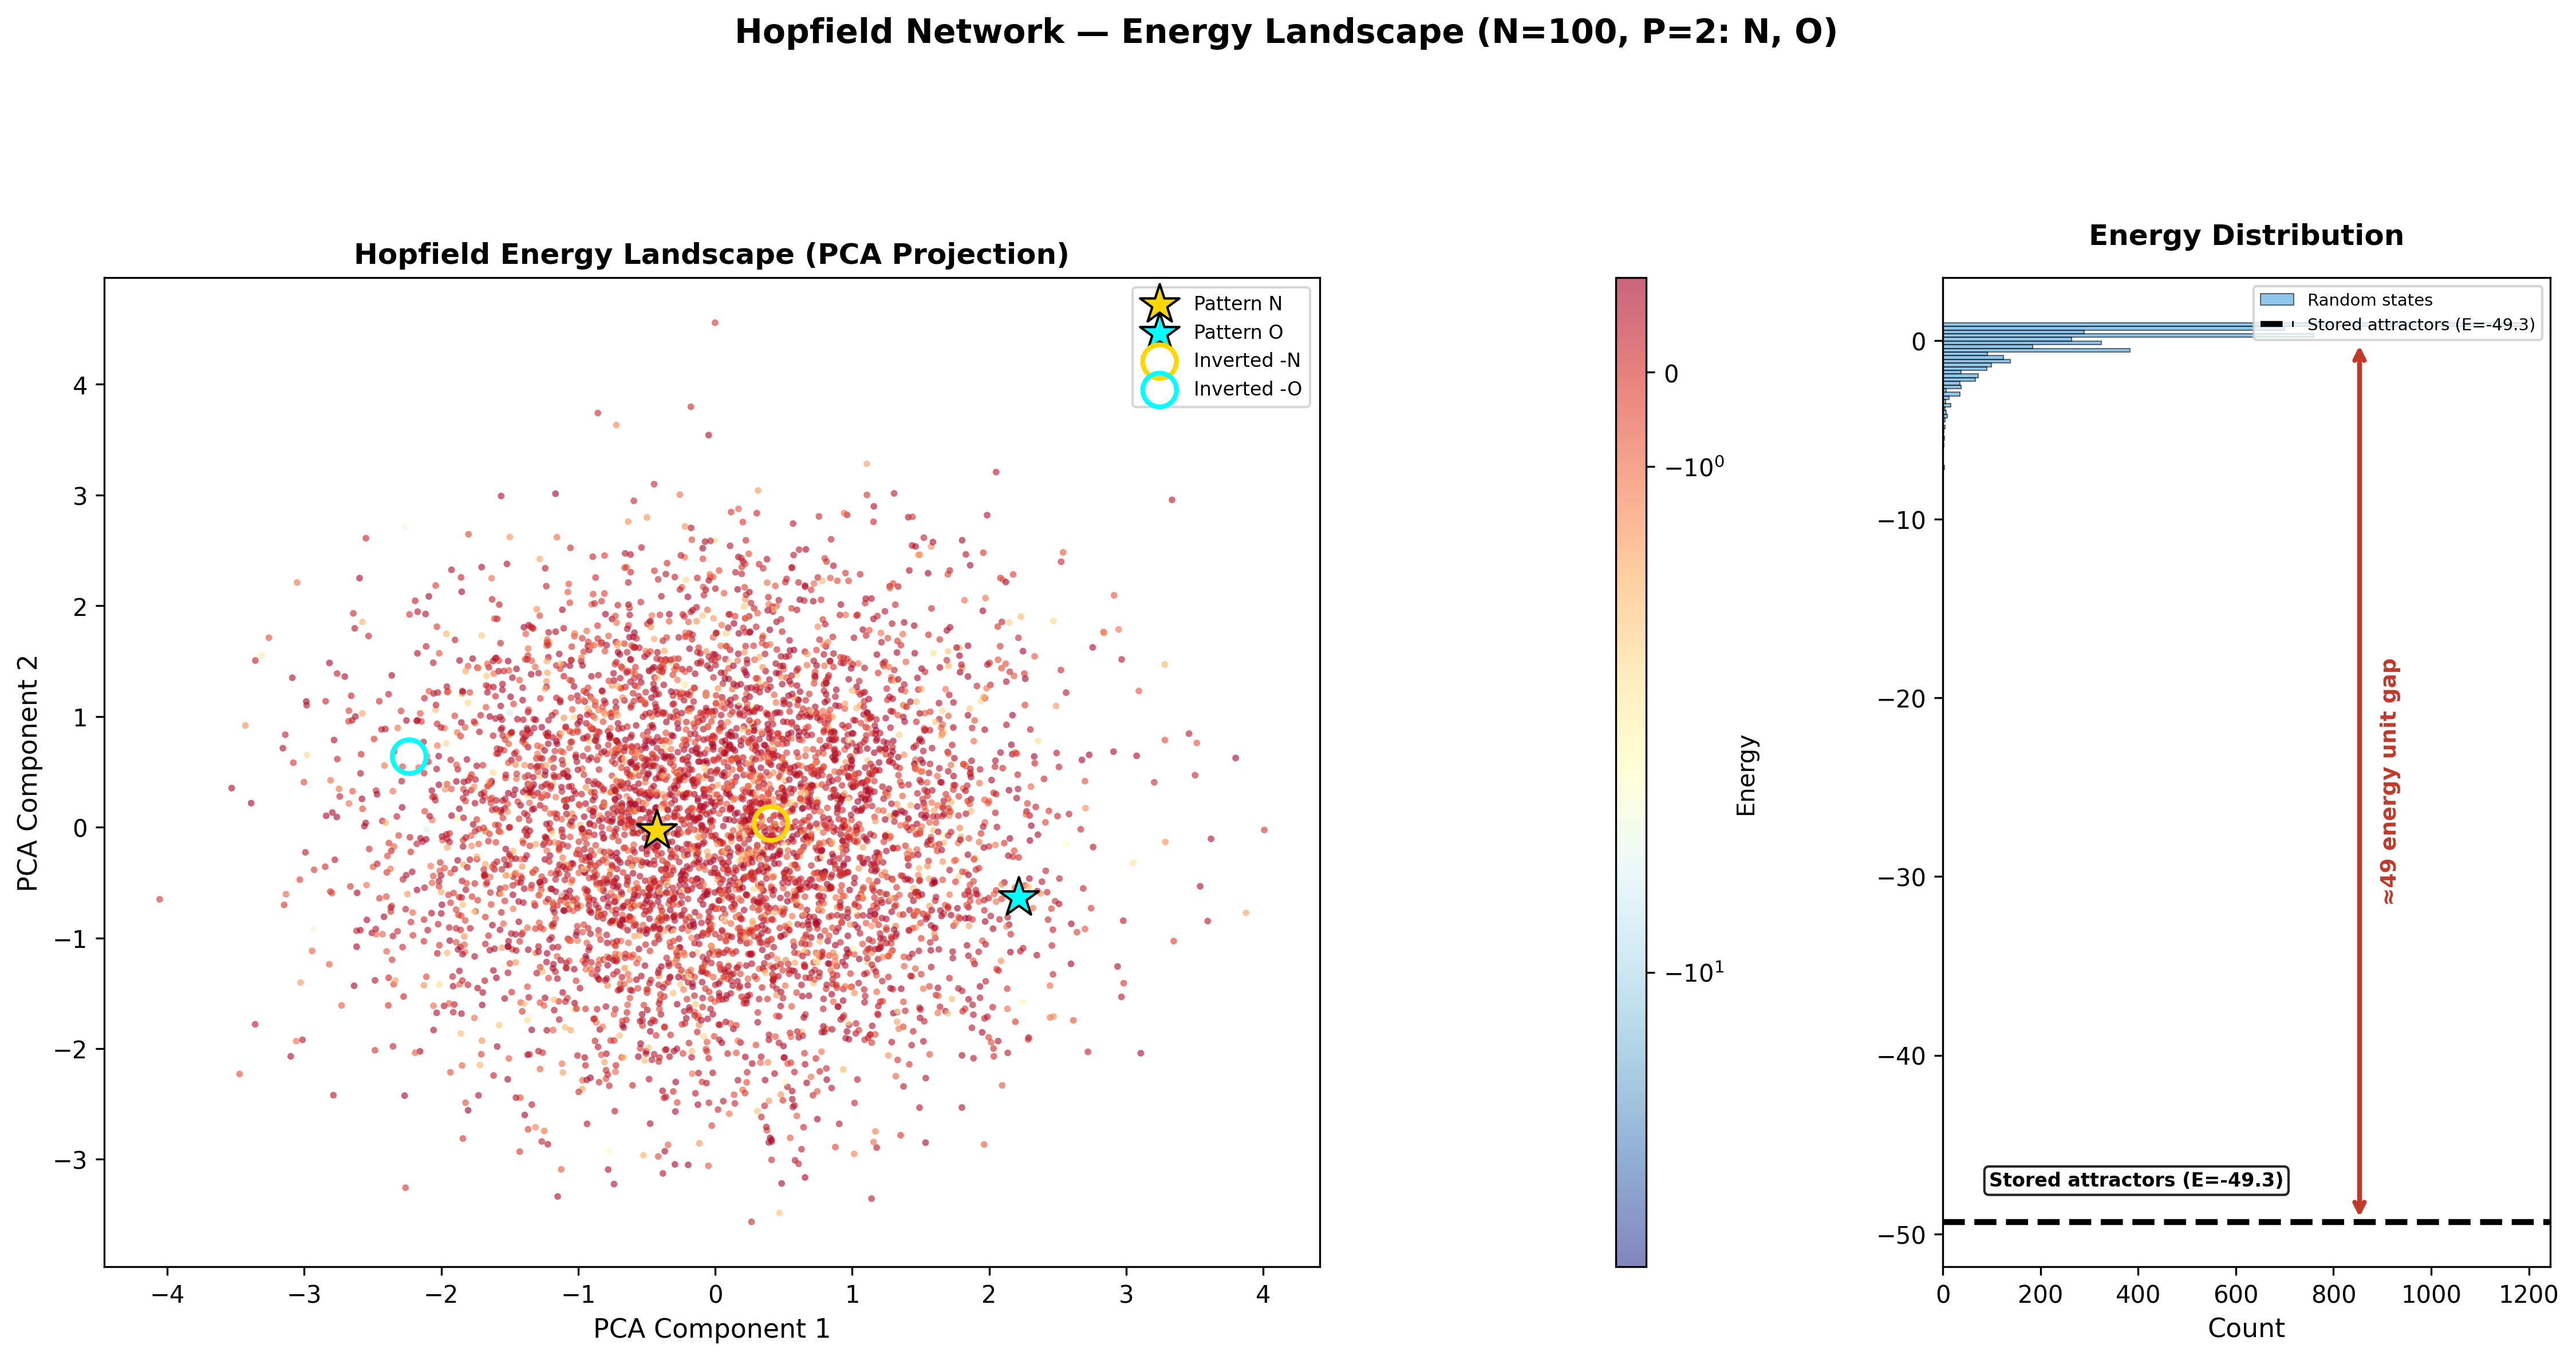
\includegraphics[width=0.85\textwidth]{figures/exp3_energy_landscape.png}
    \caption{Energy landscape of a 2-pattern network (N, O) projected to 2D
    via PCA\@. Left: 5000 random states scatter (colored by symlog energy)
    with stored patterns (stars) and their inverses (open circles). Right:
    energy histogram revealing the ${\sim}49$ unit gap between random
    configurations (clustered near $E \approx 0$) and stored attractors
    ($E = -49.3$, dashed line).}
    \label{fig:landscape}
\end{figure*}

Figure~\ref{fig:landscape} reveals two distinct populations of
configurations. In the PCA scatter (left), the 5000 random states form a
dense cloud centered near the origin, with the stored patterns and their
inverses located at the periphery. The true depth of the energy wells is more
clearly visible in the right panel: the random state distribution peaks just
below $E = 0$, while the stored attractors sit at $E = -49.3$, a gap of
approximately 49 energy units. This dramatic separation explains why the
network is so robust to corruption---moving from a random configuration to a
stored pattern releases enormous amounts of energy, and the gradient pulling
the system toward the stored state is correspondingly steep.

\begin{figure}[H]
    \centering
    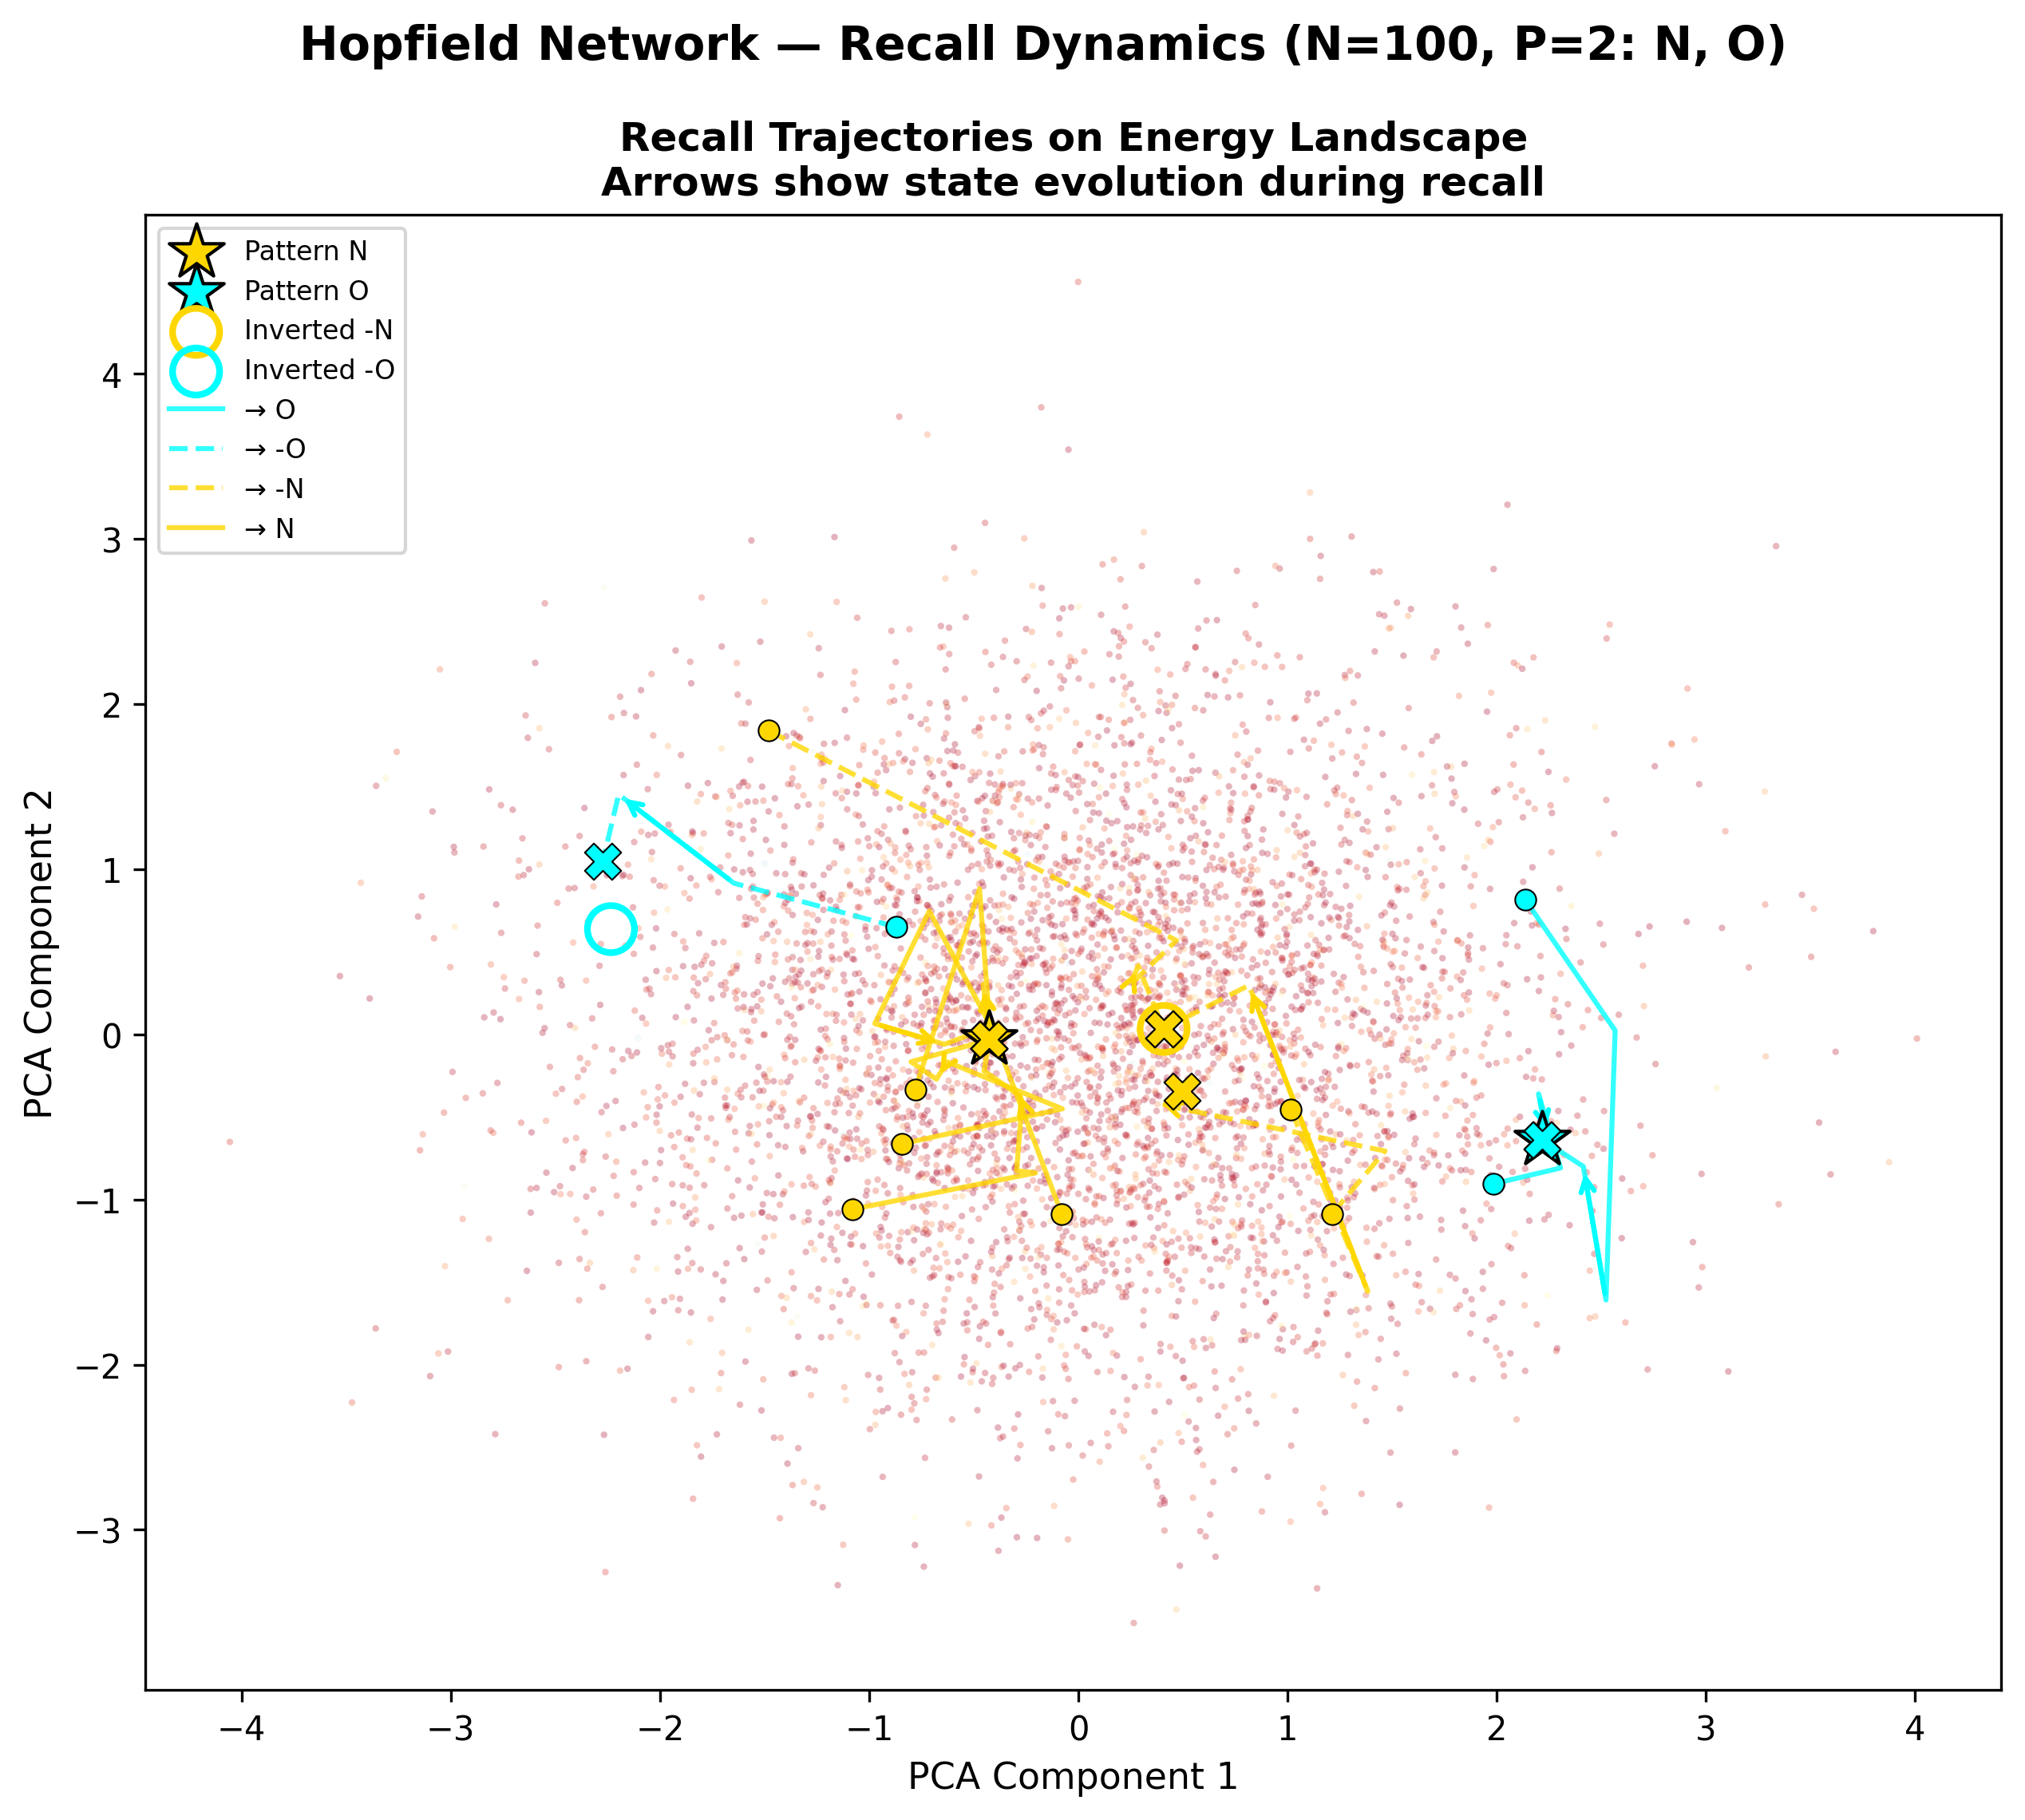
\includegraphics[width=\columnwidth]{figures/exp3_recall_trajectories.png}
    \caption{Recall trajectories on the N--O energy landscape. Arrows trace
    how 10 random initial states evolve during asynchronous recall, converging
    to one of four attractors: N, O, $-$N, or $-$O\@. The visit distribution
    across all four basins is consistent with the expected $\Z_2$ symmetry.}
    \label{fig:trajectories}
\end{figure}

Figure~\ref{fig:trajectories} plots actual recall trajectories superimposed on
this landscape. The arrows definitively trace gradient descent. The
deterministic asynchronous update rule guarantees that every single transition
must move to an equal or lower energy contour. This visualizes the Lyapunov
property in action: associative memory is literally the physics of a marble
rolling downhill.

\subsection{The Ising--Hopfield Isomorphism}
\label{sec:isomorphism}

The centerpiece of this phase is the formal demonstration that magnetic
equilibration and memory recall are identical computational processes. As
shown in Figure~\ref{fig:isomorphism}, the trajectory of a Hopfield network
correcting a corrupted image implements the same energy-minimization principle
as an Ising lattice relaxing toward equilibrium, with the deterministic
asynchronous update rule serving as the zero-temperature limit of Metropolis
dynamics. Both systems descend a Lyapunov function defined by quadratic spin
interactions; the distinction lies only in the source of the coupling matrix
(physical exchange constant $J$ versus learned Hebbian weights $W_{ij}$).

\begin{figure*}[t]
    \centering
    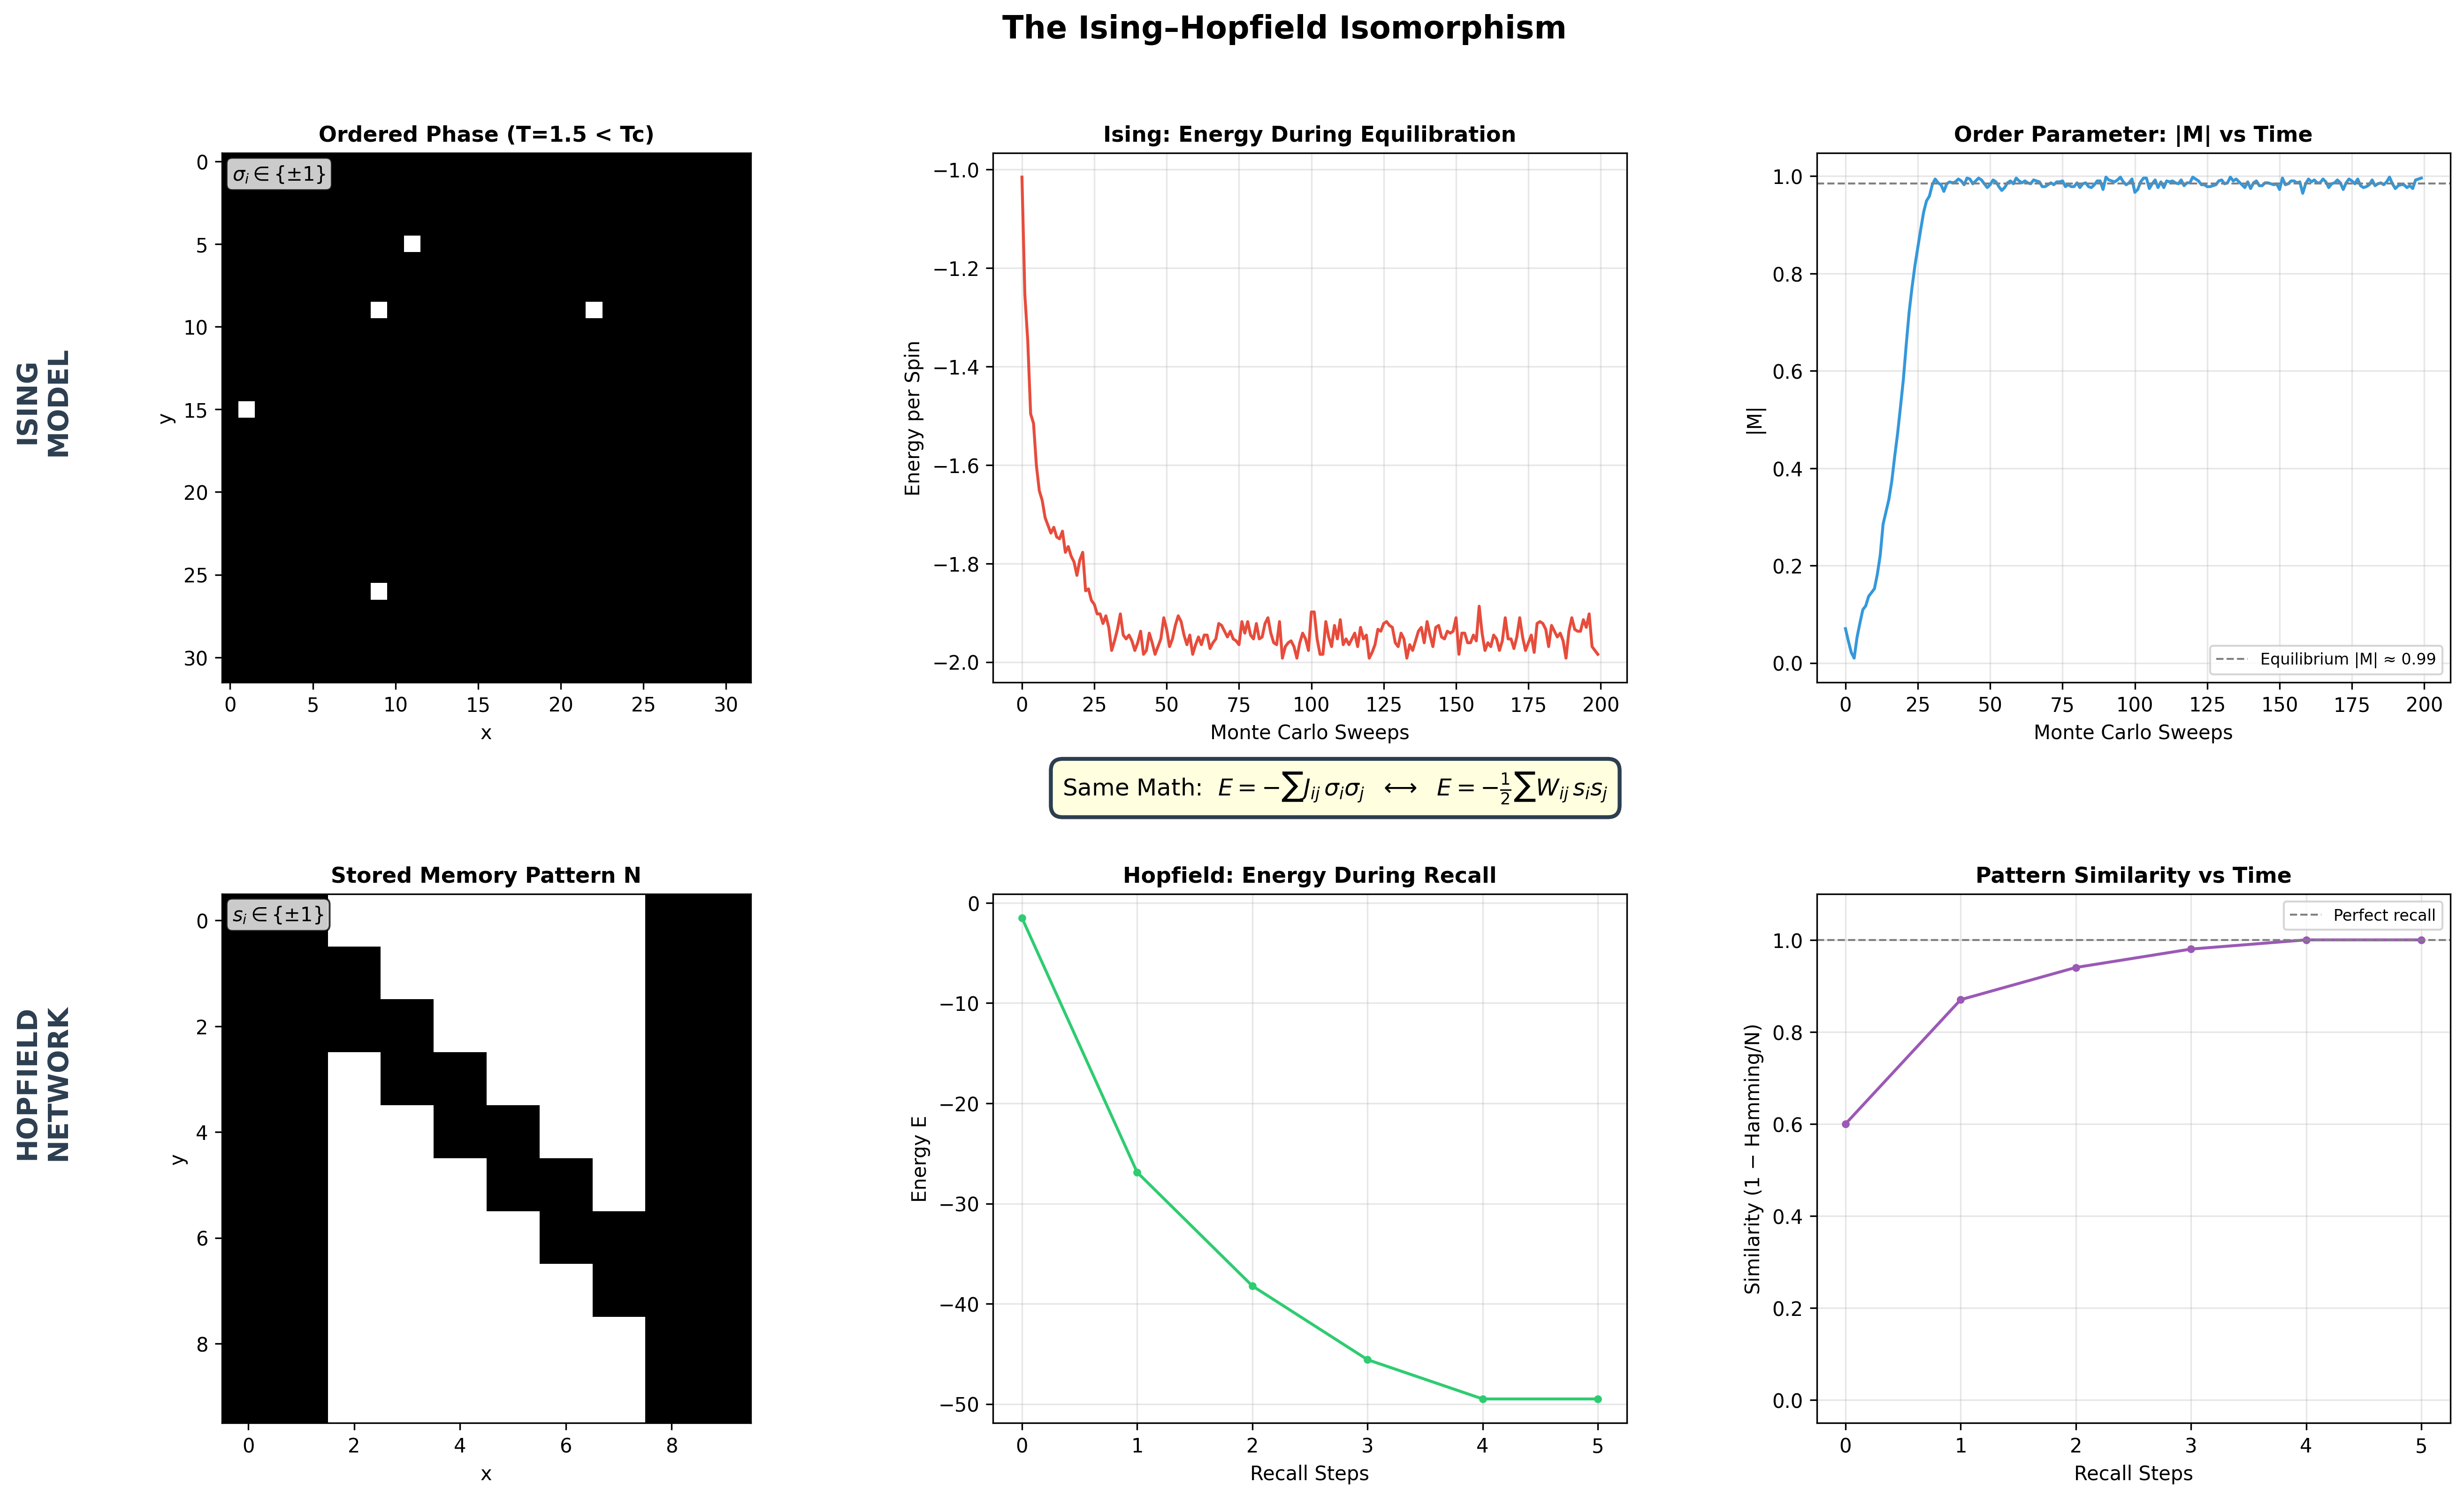
\includegraphics[width=0.85\textwidth]{figures/comparison_ising_hopfield.png}
    \caption{The central result. (Top row) Ising model equilibration: spin
    lattice, energy descent, order parameter convergence. (Bottom row)
    Hopfield recall: stored pattern, energy descent, pattern similarity
    convergence. Both systems minimize the same form of energy function.}
    \label{fig:isomorphism}
\end{figure*}

In the Ising model, the system descends an energy gradient defined by a fixed,
uniform coupling $J$, driving the lattice toward a state of uniform
magnetization. In the Hopfield network, the system descends a heavily
sculpted energy gradient defined by a learned matrix $W$, driving the network
toward a specific, complex configuration.

We summarize this fundamental equivalence in Table~\ref{tab:isomorphism}.

\begin{table}[H]
    \centering
    \caption{The Ising--Hopfield isomorphism: a formal mapping between
    physical and computational quantities.}
    \label{tab:isomorphism}
    \begin{tabular}{ll}
        \toprule
        \textbf{Ising Model} & \textbf{Hopfield Network} \\
        \midrule
        Spin $\sigma_i \in \{\pm1\}$ & Neuron state $s_i \in \{\pm1\}$ \\
        Exchange coupling $J$ & Synaptic weight $W_{ij}$ \\
        External field $B$ & Input bias $\theta_i$ \\
        Ground state & Stored memory pattern \\
        Thermal fluctuations & Stochastic updates \\
        Equilibration & Memory recall \\
        \bottomrule
    \end{tabular}
\end{table}

The implication is that the Hopfield network does not merely
metaphorically resemble physics; it \emph{is} an Ising model with a
heterogeneous coupling topology. The ability to retrieve information is an
emergent property of statistical mechanics.

% ===========================================================================
% SECTION 5: DISCUSSION
% ===========================================================================
\section{Discussion}
\label{sec:discussion}

\subsection{Quantitative Agreement with Theory}
\label{sec:quant_agreement}

Our experimental results validate the core operating principles of the
Hopfield architecture. The network demonstrates robust single-pattern recall,
maintaining a $68.0\% \pm 6.7\%$ strict success rate even when a quarter of
the input data is destroyed.

However, the capacity analysis (Figure~\ref{fig:capacity}) underscores a
critical limitation of the standard Hebbian learning rule. While the
Amit--Gutfreund--Sompolinsky limit predicts a theoretical capacity of
$\sim 13.8$ patterns for $N=100$, our network's accuracy crosses below 50\%
between $P=3$ (68.7\%) and $P=5$ (48.8\%)---less than half the theoretical
limit. This is not a failure of the theory, but rather a consequence of our
training data. The theoretical $0.138N$ limit assumes purely orthogonal,
random patterns. Natural data---like the letters of the alphabet---are highly
correlated. This correlation induces structural interference in the weight
matrix, raising the energy floor of the attractors and substantially reducing
the effective capacity.

Additionally, the spurious states analysis (Section~\ref{sec:spurious})
yielded a 201-vs-201 split between stored and inverted convergences,
consistent with the $\Z_2$ symmetry that underlies both Hopfield networks and
the original Ising model. While this symmetry is mathematically guaranteed by
the zero-bias Hebbian energy function, observing near-exact equipartition in
a finite sample provides empirical validation of the simulation dynamics.

\subsection{Recall as Physical Equilibration}
\label{sec:recall_equilibration}

The trajectories mapped in Figure~\ref{fig:trajectories} and the direct
comparison in Figure~\ref{fig:isomorphism} confirm our central thesis:
associative memory is energy minimization. The network does not ``search'' for
a memory through algorithmic logic; it relaxes into it through thermodynamic
necessity. The computational problem of pattern recognition is solved by
mapping the desired patterns into the ground states of a simulated physical
system.

\subsection{Limitations}
\label{sec:limitations}

While theoretically elegant, the classical Hopfield network presented here
suffers from several limitations. The $0.138N$ capacity constraint heavily
restricts practical utility. The Hebbian learning rule struggles severely with
correlated data. Most importantly, the network contains only visible
units---it is completely deterministic and operates purely as a retrieval
system, entirely incapable of generating new representations or inferring
latent features.

% ===========================================================================
% SECTION 6: CONCLUSION
% ===========================================================================
\section{Conclusion: Bridging to Phase 2.5}
\label{sec:conclusion}

Phase~2 has successfully achieved its core objectives, establishing the
precise mathematical bridge between the physics of equilibrium thermodynamics
and the engineering of associative memory. This paper marks the transition
from purely physical simulation to biologically-inspired computation.

\subsection{The Limitation: From Recall to Generation}
\label{sec:limitation_recall}

The Hopfield architecture, lacking hidden units, cannot model the latent
structure of complex data. It can only recall what it has explicitly memorized.
The deterministic update rule, while guaranteeing convergence, traps the
system in the nearest local minimum---a desirable property for memory
retrieval, but a fundamental obstacle for generative modeling.

\subsection{The Solution: Hidden Units and Stochasticity}
\label{sec:solution_rbm}

To transcend memorization and achieve true \emph{generation}, we must
introduce two missing elements: unobserved latent variables to capture complex
hierarchical features, and thermal stochasticity to allow the system to escape
local minima and sample from a probability
distribution~\cite{ackley1985,hinton2006}. This natural evolution---adding
hidden units and temperature to the Hopfield network---yields the Restricted
Boltzmann Machine (RBM).

\subsection{Summary of Achievements}
\label{sec:summary}

Phase~2 has successfully accomplished all stated objectives:
\begin{itemize}
    \item[$\checkmark$] Implemented Hebbian-trained Hopfield network with
    asynchronous recall dynamics
    \item[$\checkmark$] Quantified single-pattern robustness ($68.0\% \pm
    6.7\%$ strict recall at 25\% corruption)
    \item[$\checkmark$] Mapped storage capacity behavior, observing collapse
    well below the AGS theoretical limit due to pattern correlations
    \item[$\checkmark$] Identified and classified spurious attractors via
    500-trial random-initialization analysis
    \item[$\checkmark$] Observed empirical $\Z_2$ equipartition (201/201
    stored vs.\ inverted convergences), consistent with theoretical symmetry
    \item[$\checkmark$] Visualized the energy landscape via PCA projection,
    revealing $\sim$49 unit energy gap between random states and stored
    attractors
    \item[$\checkmark$] Established the formal Ising--Hopfield isomorphism
    with side-by-side dynamical comparison
\end{itemize}

\subsection{Future Directions}
\label{sec:future}

Phase~2.5 will extend the Hopfield architecture in two directions
simultaneously:
\begin{itemize}
    \item \textbf{Hidden units:} introducing latent variables yields the
    Boltzmann Machine, enabling hierarchical feature representation.
    \item \textbf{Stochasticity:} replacing deterministic sign updates with
    Glauber dynamics at finite temperature allows the system to escape local
    minima and sample from a probability distribution.
    \item \textbf{Tractability through restriction:} the Restricted Boltzmann
    Machine (bipartite visible-hidden graph) makes the resulting model
    trainable via Contrastive Divergence.
    \item \textbf{Beyond Phase 2.5:} Stacked RBMs lead to Deep Belief
    Networks, opening potential connections to broader frameworks in
    statistical field theory that remain to be explored in later phases.
\end{itemize}

% ===========================================================================
% CODE AND DATA AVAILABILITY
% ===========================================================================
\section*{Code and Data Availability}

The complete simulation code, analysis scripts, and raw experimental data
(including all CSV files referenced in this paper) are available in the
project repository at:
\url{https://github.com/YehiaGewily/Physics-AI-Bridge}

% ===========================================================================
% ACKNOWLEDGMENTS
% ===========================================================================
\section*{Acknowledgments}

The authors gratefully acknowledge the YouTube channel \emph{ScienceClic
English} for providing the theoretical inspiration through their series on
``The Physics of A.I.'', which served as the initial catalyst for this
research project. The five stored memory patterns N, O, V, E, R spell
``NOVER'', the name of the authors' AI-driven media production startup.

% ===========================================================================
% REFERENCES
% ===========================================================================
\bibliographystyle{ieeetr}
\bibliography{references}

\end{document}
